\scanpage{76}
\noindent Soit donc \(U_i\) un recouvrement affine de \(X_0\), et
\[
 e\in H^{0^{(\mathrm{alg})}}(X_0,\mathscr{E}xt^1(K,\mathscr{N}))
\]
représenté par des classes d'isomorphies (algébriques) d'extensions
\makebox[2em][c]{\raisebox{0.8ex}[0pt][0pt]{\parbox[c]{2em}{\figure{%
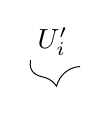
\begin{tikzpicture}[x=1mm,y=1mm,baseline=0pt]
\node[inner sep=0pt,anchor=south] at (2.8,3.8) {$\inserted{U'_i}$};
\draw[line width=0.35pt] (0.0,3.3)
 .. controls (-0.3,1.5) and (1.1,1.3) .. (1.8,1.1)
 .. controls (2.7,0.8) and (2.9,0.5) .. (3.3,0.0)
 .. controls (3.7,1.4) and (4.8,2.4) .. (6.3,2.5);
\end{tikzpicture}%
}}}} de \(U_i\) par \(\mathscr{N}\mid U_i\), classes d'isomorphies qui se recollent :

\[
 \text{soit }\unsure{\eta|n}_{ij}\text{ un isomorphisme}\qquad
 U'_j\mid U_i\cap U_j
 \xrightarrow{\sim}
 U'_{\unsure{i|j|k}}\mid U_i\cap U_j\ .
\]

L'obstruction à construire des \(\eta_{ij}\) \deleted{d}tels que \(\eta_{ij}\eta_{jk}=\eta_{ik}\) est donné par \(d_2\eta\) où \(d_2\) est une certaine flèche
\[
 d_2:H^0(X_0,\mathscr{E}xt^1(K,\mathscr{N}))\longrightarrow
 H^2(X_0,\mathscr{H}om(K,\mathscr{N}))
\]

La même construction marche dans le cas analytique, et on conclut par une nouvelle application de GAGA.

\uline{Rmq} 1 : itou pour les espaces algébriques, espaces rigides analytiques ; schémas formels

\deleted{\uline{\unsure{Rmq 2|Rmqs}}} :

\noindent\hfill Bien à toi\\
% Signature written on an upward-slanting line.
\null\hfill P. Deligne\\
\margin{\vspace*{3em}\figure{\unsure{%
\begin{tikzpicture}[x=1mm,y=1mm]
\fill (-0.20,-0.05)
 .. controls (-0.23,0.10) and (-0.10,0.20) .. (0.04,0.18)
 .. controls (0.21,0.18) and (0.25,0.05) .. (0.17,-0.09)
 .. controls (0.07,-0.19) and (-0.14,-0.18) .. (-0.20,-0.05) -- cycle;
\fill (0.62,1.02) ellipse[x radius=0.23,y radius=0.14,rotate=48];
\end{tikzpicture}%
}}}
% archive sheet number: 75
\clearpage
